%!TEX root = ../main.tex
\section{Pure preferential attachment}\label{section:pure-preferential-attachment}

\subsection{Degree distribution: Theory}\label{subsection:ppa-degree-distribution}
The master equation that describes the evolution of the BA model is given by

\begin{equation}
	n(k, t+1) = n(k, t) + m \Pi(k-1, t)n(k-1, t) - m \Pi(k, t)n(k, t) + \delta_{k,m}
	\label{eq:master}
\end{equation}
where $k$ is the total degree of a vertex, $n(k, t)$ is the number of nodes at time $t$ with total degree $k$, and the probability $\Pi$ for choosing the existing vertex depends on the model. 

In the pure preferential attachment model, we choose an existing edge with $\Pi_{pa} \propto k$, which after normalizing gives $\Pi_{pa} = k/ 2E(t)$ where $E(t)$ is the number of edges and $2E(t)$ is the normalization constant corresponding to the total degree of the network. Assuming $E(0) = mN(0)$, the number of edges at a given time $t$ is given by $E(t) = mN(t)$, so we get $\Pi = k / 2mnN(t)$. Since we are concerned with the degree distribution of the model at large $t$, we consider the long-time ansatz $n(k, t) \rightarrow N(t) p_{\infty}(k)$. 

Substituting these terms into the master equation, we obtain 
\begin{equation}
	p_{\infty}(k) = \frac{1}{2}[(k-1)p_{\infty}(k-1) - kp_{infty}(k)] + \delta_{k,m}
	\label{eq:degree-distribution-p-infinity}
\end{equation}

It is clear that $p_{\infty}(k < m) = 0$, since $m$ edges are added at every stage. So there are 2 cases to consider when solving for the above equation: $k = m$ and $k > m$. 

We first consider the case when $k > m$. In this case, $\delta_{k,m} = 0$ and we can rearrange \autoref{eq:degree-distribution-p-infinity} to get

\begin{equation}
	\frac{p_{\infty}(k)}{p_{\infty}(k+1)} = \frac{k-1}{k+2}
	\label{eq:p-infinity-k-greater-m}	
\end{equation}

To solve this equation, we can substitute in a trial solution of the form

\begin{equation}
	f(z) = A \frac{\Gamma(z+1+a)}{\Gamma(z+1+b)}
	\label{eq:trial-solution}
\end{equation}
where $\Gamma(z)$ is the Gamma function, which is an extension of the factorial function, with its argument shifted by one, to all real and complex nnumbers except the non-positive integers. Its central property is that
\begin{equation}
	\Gamma(z+1) = z \Gamma(z),\,\, \Gamma(1) = 1.
	\label{eq:gamma-function-property}
\end{equation}

Substituting the trial solution in \autoref{eq:trial-solution} gives
\begin{equation}
	\frac{A \Gamma(z+1+a)}{\Gamma(z+1+b)} \times \frac{\Gamma(z+b)}{A \Gamma(z+a)}
\end{equation}
which indeed simplifies to give $(z+a) / (z+b)$, using the the property in \autoref{eq:gamma-function-property} that $\Gamma(z+a+1) / \Gamma(z+a) = z+a$. 

Substituting $a = -1$ and $b=2$, we get the solution for \autoref{eq:p-infinity-k-greater-m} in terms of $A$ and the Gamma function:

\begin{equation}
	p_{\infty}(k) = A \frac{\Gamma(k)}{\Gamma(k+3)}
\end{equation}
which simplifies to 
\begin{equation}
	p_{\infty}(k) = \frac{A}{k(k+1)(k+2)}.
	\label{eq:p-infinity-solution-unknown-A}
\end{equation}

For the second case of $k = m$, \autoref{eq:degree-distribution-p-infinity} becomes 
\begin{equation}
	p_{\infty}(m) = \frac{1}{2}[(m+1)p_{\infty}(m-1) - mp_{\infty}(m)] + 1. 
	\label{eq:p-infinity-k-equals-m}
\end{equation}
However, we already know that $p_{\infty}(k < m) = 0$, that is, $p_{\infty}(m-1) = 0$. Using this, and rearranging \autoref{eq:p-infinity-k-equals-m}, we get 

\begin{equation}
	p_{\infty}(m) = \frac{2}{m+2}.
	\label{p-infinity-normalization}
\end{equation}

Substituting $k = m$ and \autoref{p-infinity-normalization} into \autoref{eq:p-infinity-solution-unknown-A}, we get 

\begin{equation}
	\frac{A}{m(m+1)(m+2)} = \frac{2}{m+2}, 
\end{equation}
giving us the constant $A$ as
\begin{equation}
	A = 2m(m+1).
	\label{eq:normalization-constant}
\end{equation}

For this constant to be physically reasonable, we need to check that the probability satisfies normalization, that is, we need to prove
\begin{equation}
	\sum_{k=m}^\infty p_{\infty}(k) = 2m(m+1)\sum_{k=m}^\infty \frac{1}{k(k+1)(k+2)} = 1. 
	\label{eq:normalization-criteria}
\end{equation}

The term in the summation of \autoref{eq:normalization-criteria} can be expanded as a partial fraction:
\begin{equation}
	\sum_{k=m}^\infty \frac{1}{k(k+1)(k+2)} = \sum_{k=m}^\infty \frac{1}{2k} - \sum_{k=m}^\infty \frac{1}{k+1} + \sum_{k=m}^\infty \frac{1}{2(k+2)}
	\label{eq:partial-fractions}
\end{equation}

By writing out the first few terms of each summation, we can see that most terms cancel:

\begin{equation}
\setlength{\arraycolsep}{0pt}% no padding
\newcolumntype{B}{>{{}}c<{{}}}
\begin{array}{ B l B l B l B l B l B}
	\frac{1}{2m} & {}-{} &\frac{1}{m+1} & {}+{} & \cancel{\frac{1}{2(m+2)}} & \\
	& {}+{} & \frac{1}{2(m+1)} & {}-{} &\cancel{\frac{1}{m+2}} & {}+{} &\cancel{\frac{1}{m+3}} \\
	& & & {}+{} & \cancel{\frac{1}{2(m+2)}} & {}-{} & \cancel{\frac{1}{m+3}} & {}+{} &\frac{1}{2(m+4)} \\
	& & & & & {}+{}& \cancel{\frac{1}{2(m+3)}} & {}-{} & \frac{1}{m+4} & {}+{} & \frac{1}{2(m+5)} \\
	& & & & & & & {}+{}& ...\\
\end{array}
\label{eq:summation-cancel}
\end{equation}
and from the remaining terms we get the relation in \autoref{eq:normalization-criteria}
\begin{equation}
	 \sum_{k=m}^\infty p_{\infty}(k) = 2m(m+1)\left ( \frac{1}{2m} - \frac{1}{m} + \frac{1}{2(m+1)} \right ) = 2m(m+1) \frac{1}{2m(m+1)} = 1
	 \label{eq:normalization-satisfied}
\end{equation}

Hence, we can confirm that the complete exact solution for the probability distribution in the long time limit is 
\begin{equation}
	p_{\infty}(k) = \frac{2m(m+1)}{k(k+1)(k+2)}.
	\label{eq:p-infinity-solution}
\end{equation}

\subsection{Degree distribution: Numerical analysis}\label{subsection:ppa-numerical-analysis}

To leverage its speed, \texttt{c++} code was used to generate graph data, while \texttt{python} was used for data analysis due to its wide range of data analysis tools, such as \texttt{numpy}, \texttt{scipy}, and \texttt{pandas}. 

There were two main concerns when doing the numerical simulation:

\begin{enumerate}
	\item What should the initial graph $G_0$ be? 
	\item Should self loops and multiple edges be allowed?
	\item Of what order should $m$ and $N$ be respectively?
\end{enumerate}

The initial graph should be negligible if $N \rightarrow \infty$. In our simulations, we assumed that the $N$ chosen was large enough for this limit to apply, so we for convenience we chose our initial graph to be an empty graph. 

Computational efficiency of our algorithm is important considering that bigger datasets give better and more reliable statistical results. To yield statistically significant results and optimize efficiency, the following algorithm was used. In this algorithm, the array $M$ holds the list of edges represented by pairs of vertices, for example, the vertices at $M[0]$ and $M[1]$ are connected, $M[2]$ and $M[3]$ are connected, and so on. In this list, the number of occurences of a vertex is equal to its degree, so it can be used as a sample pool to achieve preferential attachment. To choose $m$ neighbours for each new vertex, we then sample from $M$. This is also equivalent to choosing an edge at random and then choosing a vertex at random from the edge. 

\begin{algorithm}
\caption{Algorithm for preferential attachment}\label{alg:pa}
\begin{algorithmic}[1]
\Require{number of vertices $N$, minimum degree $m$}\Comment{$N > m$}
\State Initialize our graph $g$
\State Initialize $M$ as an empty array of length $2Nm$
\For{$v$ in [0, ..., n-1]}
	\State add new vertex to $g$
	\For{$i$ in [0, ..., m-1]}
		\State $M[2(vm + i)] \gets v$
		\State draw $r$ uniformly at random 
		\State from $[0, ..., 2(vm + i)]$\Comment{Choose random vertex from $M$}
		\State $M[2(vm + i)+1] \gets M[r]$ \Comment{Add edge between vertex $M[r]$ and $v$}
	\EndFor
\EndFor
\State
\For{$i$ in [0, ..., nm-1]}\Comment{Add all edges stored in M into the graph}
	\State Add edge $(M[2i], M[2i+1])$ to graph $g$
\EndFor
\end{algorithmic}
\end{algorithm}

Clearly this approach produces self loops and multiple edges. However, since we are concerned with the limit of $N \rightarrow \infty$, these effects are insignificant. Also, while unsatisfactory, multiple edges and self-loops do not affect our theoretical result. In the large $N$ limit, the probability of getting multiple edges or self loops is small, and so for simplicity this algorithm was used without modification. 

$N$ was mostly limited by efficiency and storage space to be $10^7$, and $m$ was chosen to vary between $1$ and $32$. 

To check that the model was implemented correctly, the degree distribution generated by the model compared checked against the \texttt{networkx} implementation of the BA model, since it is an established software package. It was verified that the degree distribution for $N = 10^5$ and different values of $m$ generated through our algorithm is highly similar to the \texttt{networkx} degree distributions. This gives confidence that the algorithm is working as expected. 

To investigate the degree distribution, the model was run for fixed $N$ but varying $m$. Several numerical runs were performed for each set of values to improve statistics. It was found that generally above $N=10^4$, finite size scaling effects are insignificant (see \autoref{subsection:pa-numerical-largest-degree}). In order to reduce finite size effects, $N=10^6$ was used. 

As $N$ is finite, there is bound to be a noisy tail at large $k$, where these degrees appeared once. To reduce the noise, 100 simulations were run for a single $m$ and the degree distribution was averaged over all runs. This can be seen in \autoref{fig:pa-fixed-n-degree-dist}. The log-binning technique \citep{Christensen:2005} was adopted to to collapse the noisy data. 

\begin{figure}
    \centering
    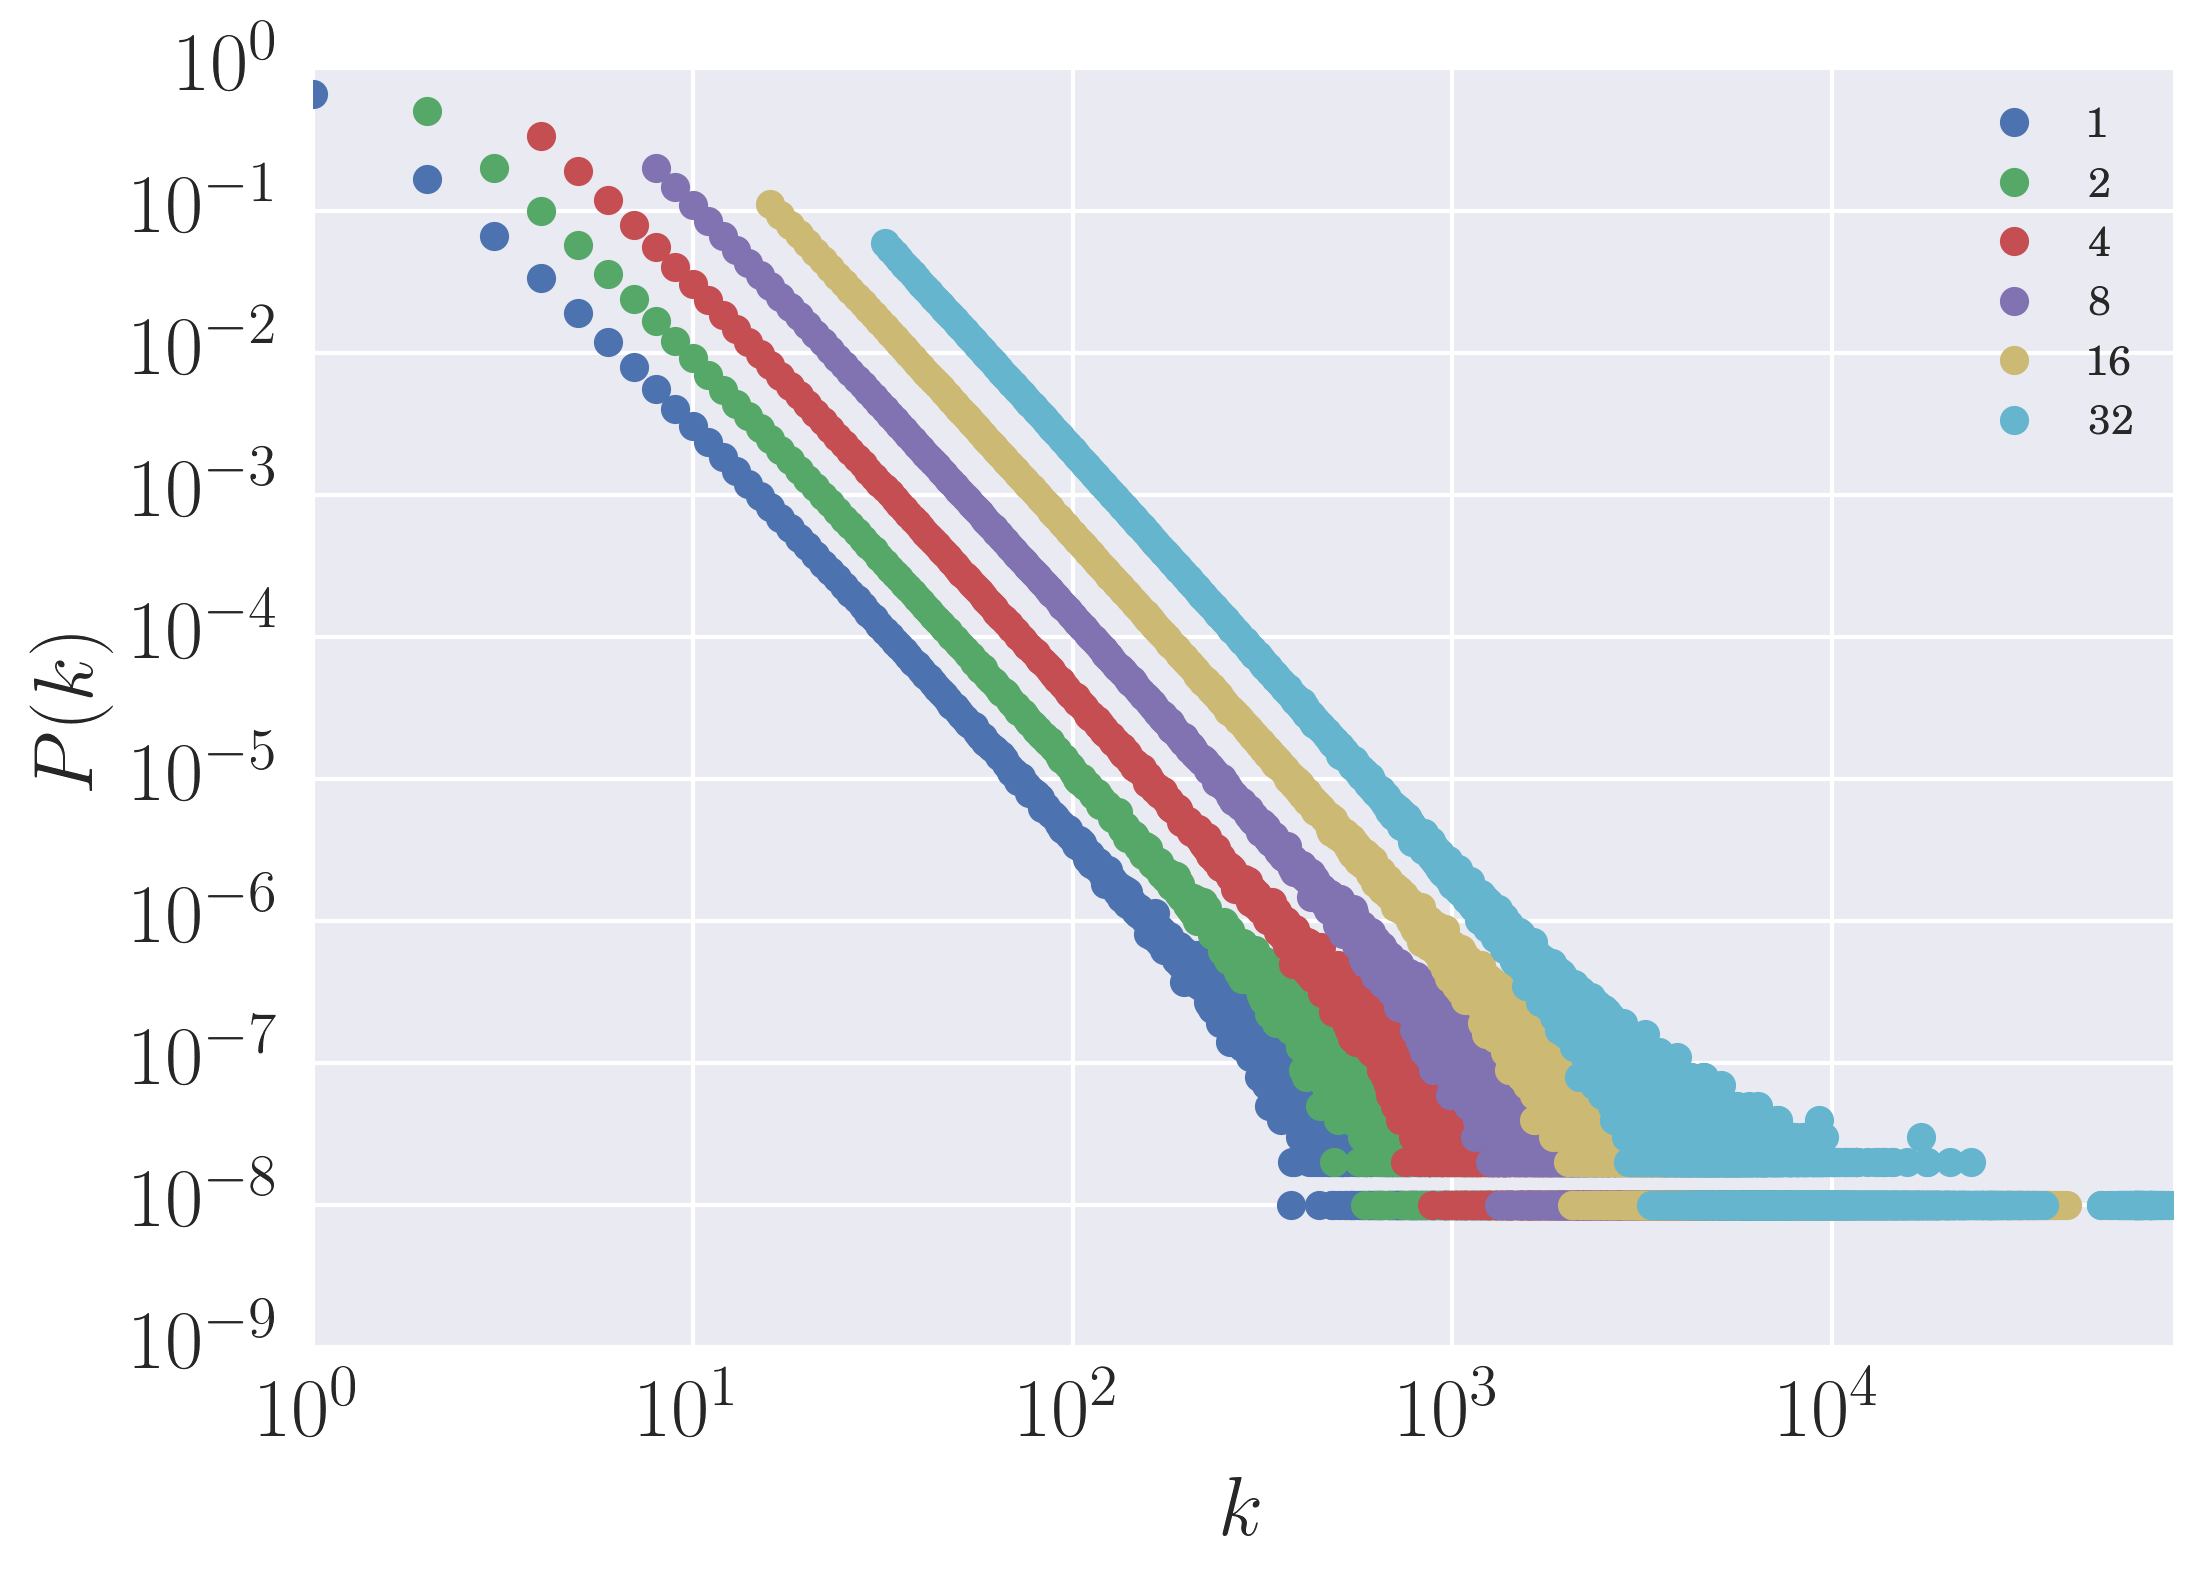
\includegraphics[height=0.5\linewidth]{img/pa-fixed-n-degree-dist}
    \caption{Raw degree distribution averaged over 100 runs for $m = 1, 2, 4, 8, 16, 32$. A noisy tail can still be seen at large $k$ due to finite sized effects. }
    \label{fig:pa-fixed-n-degree-dist}
\end{figure}

Visually, as can be seen from \autoref{fig:pa-fixed-n-logbin}, the numerical results seem to agree with the theoretical model after log-binning, until finite sized effects begin to kick in at large $k$. Alternatively, we can look at the complementary cumulative distribution function (ccdf) to observe the behaviour of the fat tail more clearly. This is shown in \autoref{fig:ccdf}. We can see that near the fat tail, the numerical ccdf goes slightly higher than the theoretical, before falling off. This is consistent across different $m$ values.

\begin{figure}
    \centering
    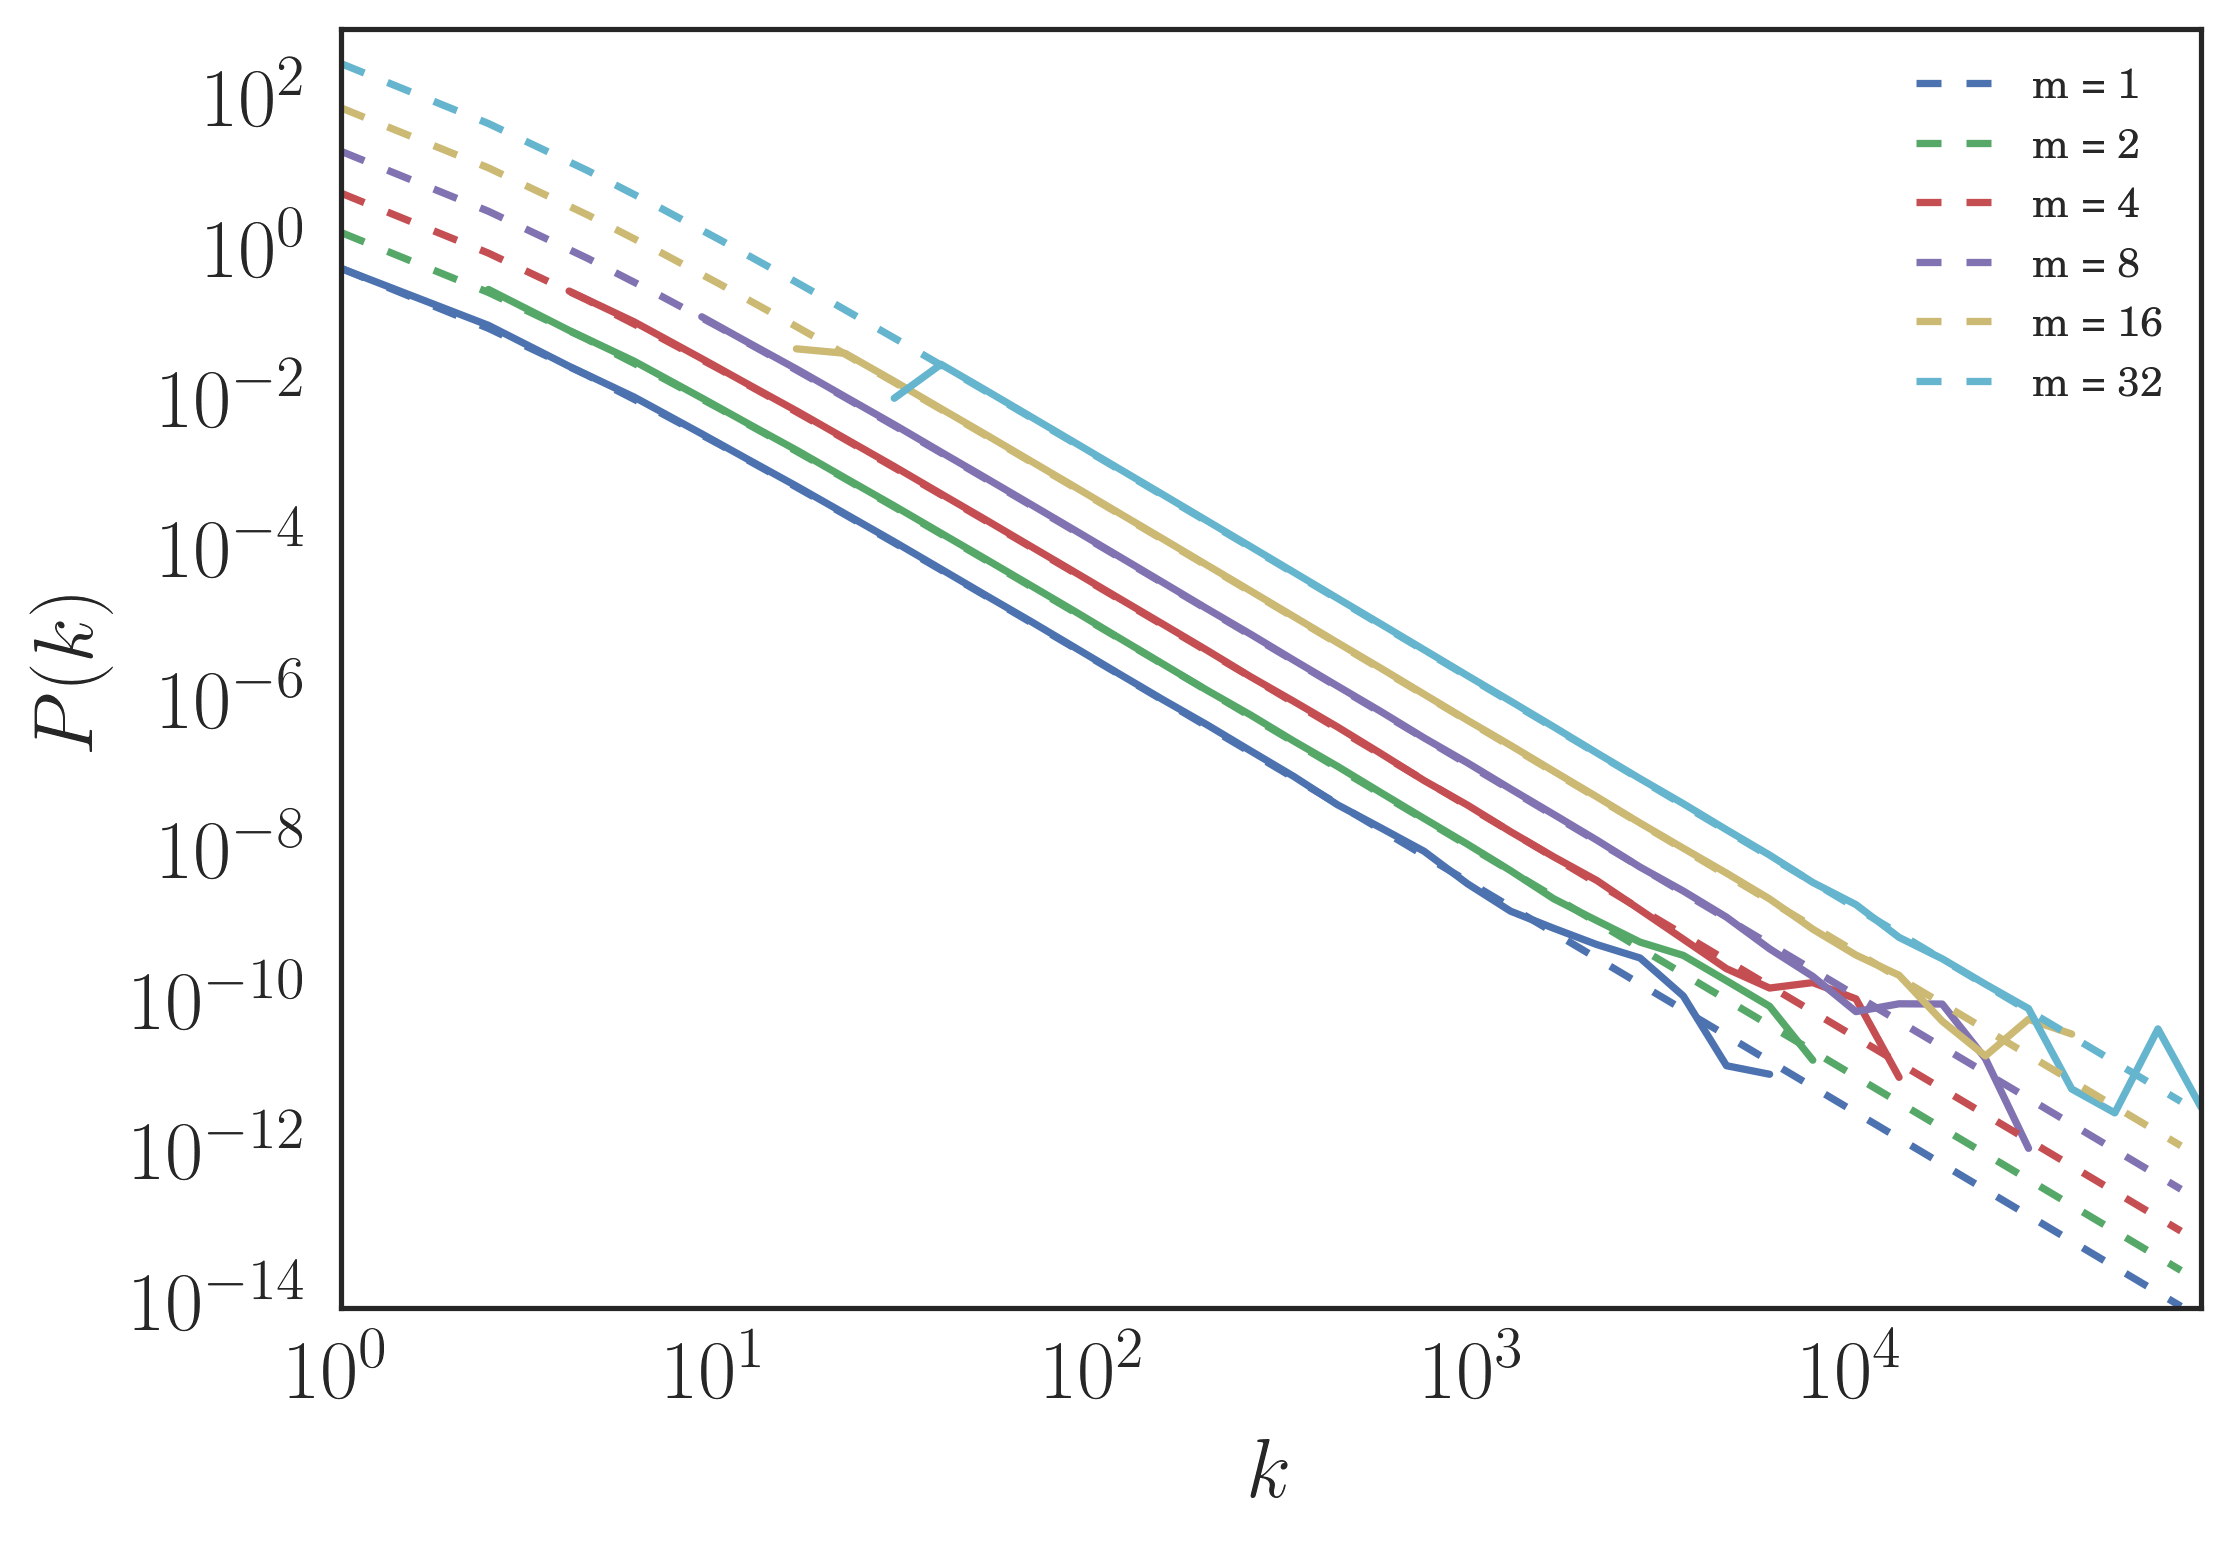
\includegraphics[height=0.5\linewidth]{img/pa-fixed-n-logbin}
    \caption{The solid lines show log-binned degree distributions for $m = 1, 2, 4, 8, 16, 32$. The dashed lines show the values predicted by the theoretical model. There is good agreement for small $k$ finite sized effects kick in. }
    \label{fig:pa-fixed-n-logbin}
\end{figure}

\begin{figure}
    \centering
    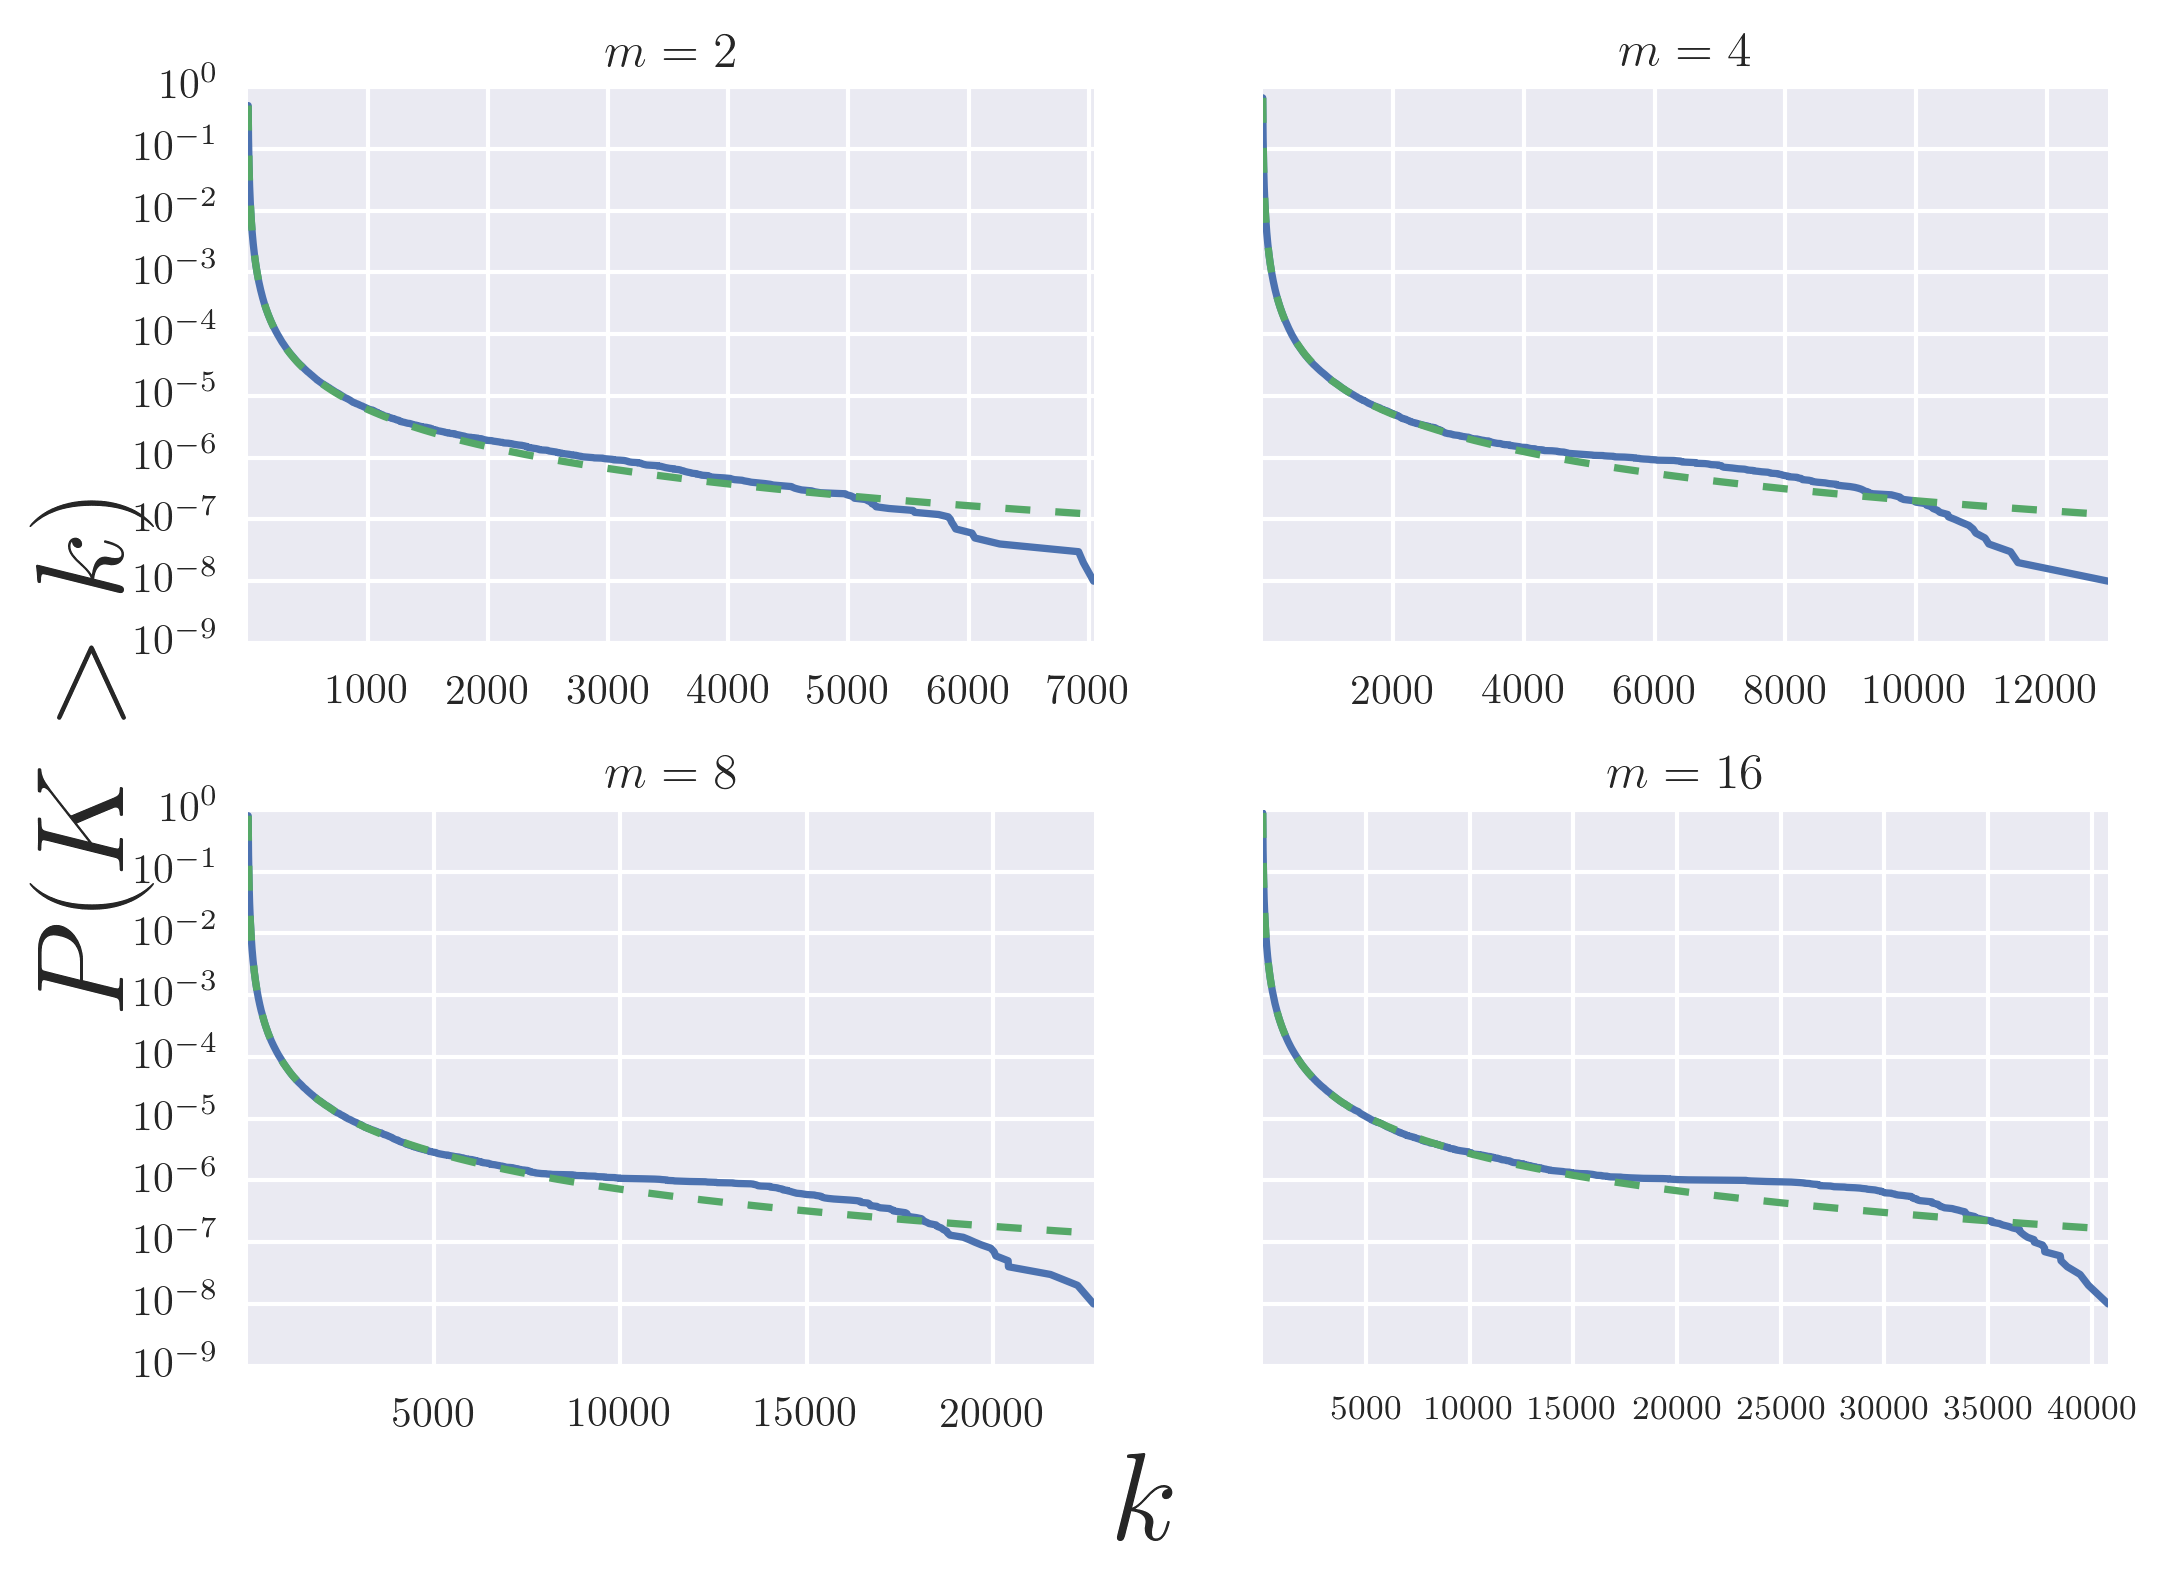
\includegraphics[height=0.7\linewidth]{img/ccdf}
    \caption{CCDF of $m=2, 4, 8, 16$, where the solid line is the numerical CCDF and the dotted line is the CCDF predicted by theory.}
    \label{fig:ccdf}
\end{figure}

A Kolmogorov-Smirnov (KS) test was used to quantify the goodness-of-fit between theory and numerical results. It is a non-parametric test that measures how far apart two distributions are, and it returns a KS-statistic that can be converted into a p-value. A smaller KS-statistic implies that the numerical data and theoretical distribution are more similar and that differences between data and model may be attributed to statistical differences, while a large KS-statistic that the model is unlikely to have been the generating function for the data. 

The table below shows the results of the KS test on $m = 1$ to $m=32$:

\begin{center}
\begin{tabular}{ c | c }
 m &  KS-statistic \\ 
 \hline
 1 & 0.000414 \\  
 2 & 0.000978 \\
 4 & 0.000744 \\
 8 & 0.000662 \\
 16 & 0.001002 \\
 32 & 0.001132 \\  
\end{tabular}
\label{table:ks-test}
\end{center}

However, these values are meaningless unless we know what kind of deviation from theoretical is considered acceptable, and at what value we should reject the null hypothesis. To answer that, we generate synthetic datasets governed by the theoretical distribution in \autoref{eq:p-infinity-solution} to measure how far they fluctuate from the reference theoretical distribution in a similar way as described by \citet{Clauset2009}, and compare the results with the simulated data. 

The synthetic datasets were generated with a lower bound of $m$ and an upper bound given by the maximum degree in the simulated dataset. If the simulated data is much further from the theoretical distribution than the typical synthetic data, then we would have grounds to reject the null hypothesis. 

For each of the synthetic datasets, we compare it to the theoretical distribution and calculate its KS-statistic. Then we define our $p$-value as the fraction of the time the resulting statistic is larger than the value for the numerical data. We can then reject the null hypothesis if $p \leq 0.1$ \citep{Clauset2009}, that is, if there is a 1 in 10 probability or less that we would, by chance, get data that agree as poorly with the model as the current data. 

Another issue to consider is the number of synthetic datasets to generate. Again, \citet{Clauset2009} suggests a useful rule: to have p-values accurate to within about $\epsilon$, we need at least $\frac{1}{4}\epsilon^{-2}$ datasets. In this project, 100 datasets were generated for each $m$, to get an accuracy of about $0.05$. 

The resulting p-values are given in the table below:
\begin{center}
\begin{tabular}{ c | c }
 m &  p-value\\ 
 \hline
 1 & 0.71 \\  
 2 & 0.45 \\
 4 & 0.50 \\
 8 & 0.58 \\
 16 & 0.71 \\
 32 & 0.46 \\  
\end{tabular}
\captionof{table}{The list of $p$-values for each $m$ for preferential attachment when compared with synthetic datasets.}
\label{table:ks-test-all}
\end{center}

Since the $p$-values for each $m$ are all larger than $0.1$, we can say it is plausible that the numerical data was drawn from the theoretical distribution. 

A point to note is that the KS test is used for continuous distributions, while our degree distribution is discrete. However, it was assumed that for large $N$, there will be values spanning a large range of $k$, hence the change in $k$ can be considered small, and the distribution can be approximated as a continuous distribution. 

A chi-squared test was also considered. The chi-squared test is a categorical test, suitable for discrete distributions, however, the test becomes invalid when the observed or expected frequencies for each category is too small, with a typical rule being that the frequencies should be at least 5 \citep{Lawrence1997}. In our numerical data, there many large values of $k$ that only appeared once, and hence this test was determined to be not suitable. 

\subsection{Largest expected degree: Theory}
The finite size of the system imposes a structural cutoff on the largest expected degree. For scale free networks, \citet{Aiello2001a} defined the maximum degree to be approximately the value above which there is less than one vertex of that degree in the graph on average, that is, $N \sum_{k = k_1}^\infty p_\infty(k) = 1$. 

Generally, it is shown \citep{Boguna2004} that for a scale free network with $p_{\infty}(k) \propto k^{\gamma}$, the largest expected degree will be

\begin{equation}
	k_1(N) \sim N^{1 / (\gamma -1)}.
	\label{eq:largest-expected-degree-research}
\end{equation}
Starting with the equation 

\begin{equation}
	N \sum_{k=k_1}^\infty p_{\infty}(k) = 1, 
	\label{eq:largest-expected-degree-criteria}
\end{equation}
we can see that this is almost identical to \autoref{eq:normalization-criteria}, just with a different factor and lower limit. Hence we have 
\begin{equation}
	2m(m+1) \frac{1}{2k_1(k_1+1)} = \frac{1}{N}.
	\label{eq:largest-expected-degree-derivation}
\end{equation}
We can then rearrange this to give us an expression for $k_1$:
\begin{equation}
	k_1 = \frac{-1 + \sqrt{1 + 4Nm(m+1)}}{2}
	\label{eq:pa-k1-expression}
\end{equation}
where the other negative solution is rejected as it is unphysical, and confirming that verifying that $k \propto N^{0.5}$. 

\subsubsection{Numerical analysis: Largest expected degree}\label{subsection:pa-numerical-largest-degree}

As can be seen from the \autoref{fig:pa-numerical-theoretical-k1}, the numerical value seems to be consistently slightly lower than the theoretical $k_1$ values. This is reasonable since numerical simulations are for finite $N$, and hence there will be an upper limit to the possible degrees that a vertex can take, while in the theoretical derivation, there is no upper limit to the possible values of $k$ that a vertex can have. By looking at the ratios of $ k_1 \text{(numerical)} / k_1 \text{(theoretical)} $ as shown in \autoref{table:pa-numerical-theoretical-ratio}, we can see that deviations are generally constant. 

By repeating numerical simulations for 100 times, we can estimate the error on $k_1$ by calculating the standard deviation for the sample and using the following formula to estimate population standard deviation:

\begin{equation}
	\sigma = \sqrt{\frac{1}{n} \sum_{i=1}^n (k_{1, i} - \bar{k}_1)^2}
	\label{eq:population-std}
\end{equation}
where $n$ is the number of repeats. In this case, $n = 100$. 

The values can be seen in \autoref{table:pa-numerical-theoretical-ratio}, 


\begin{figure}
    \centering
    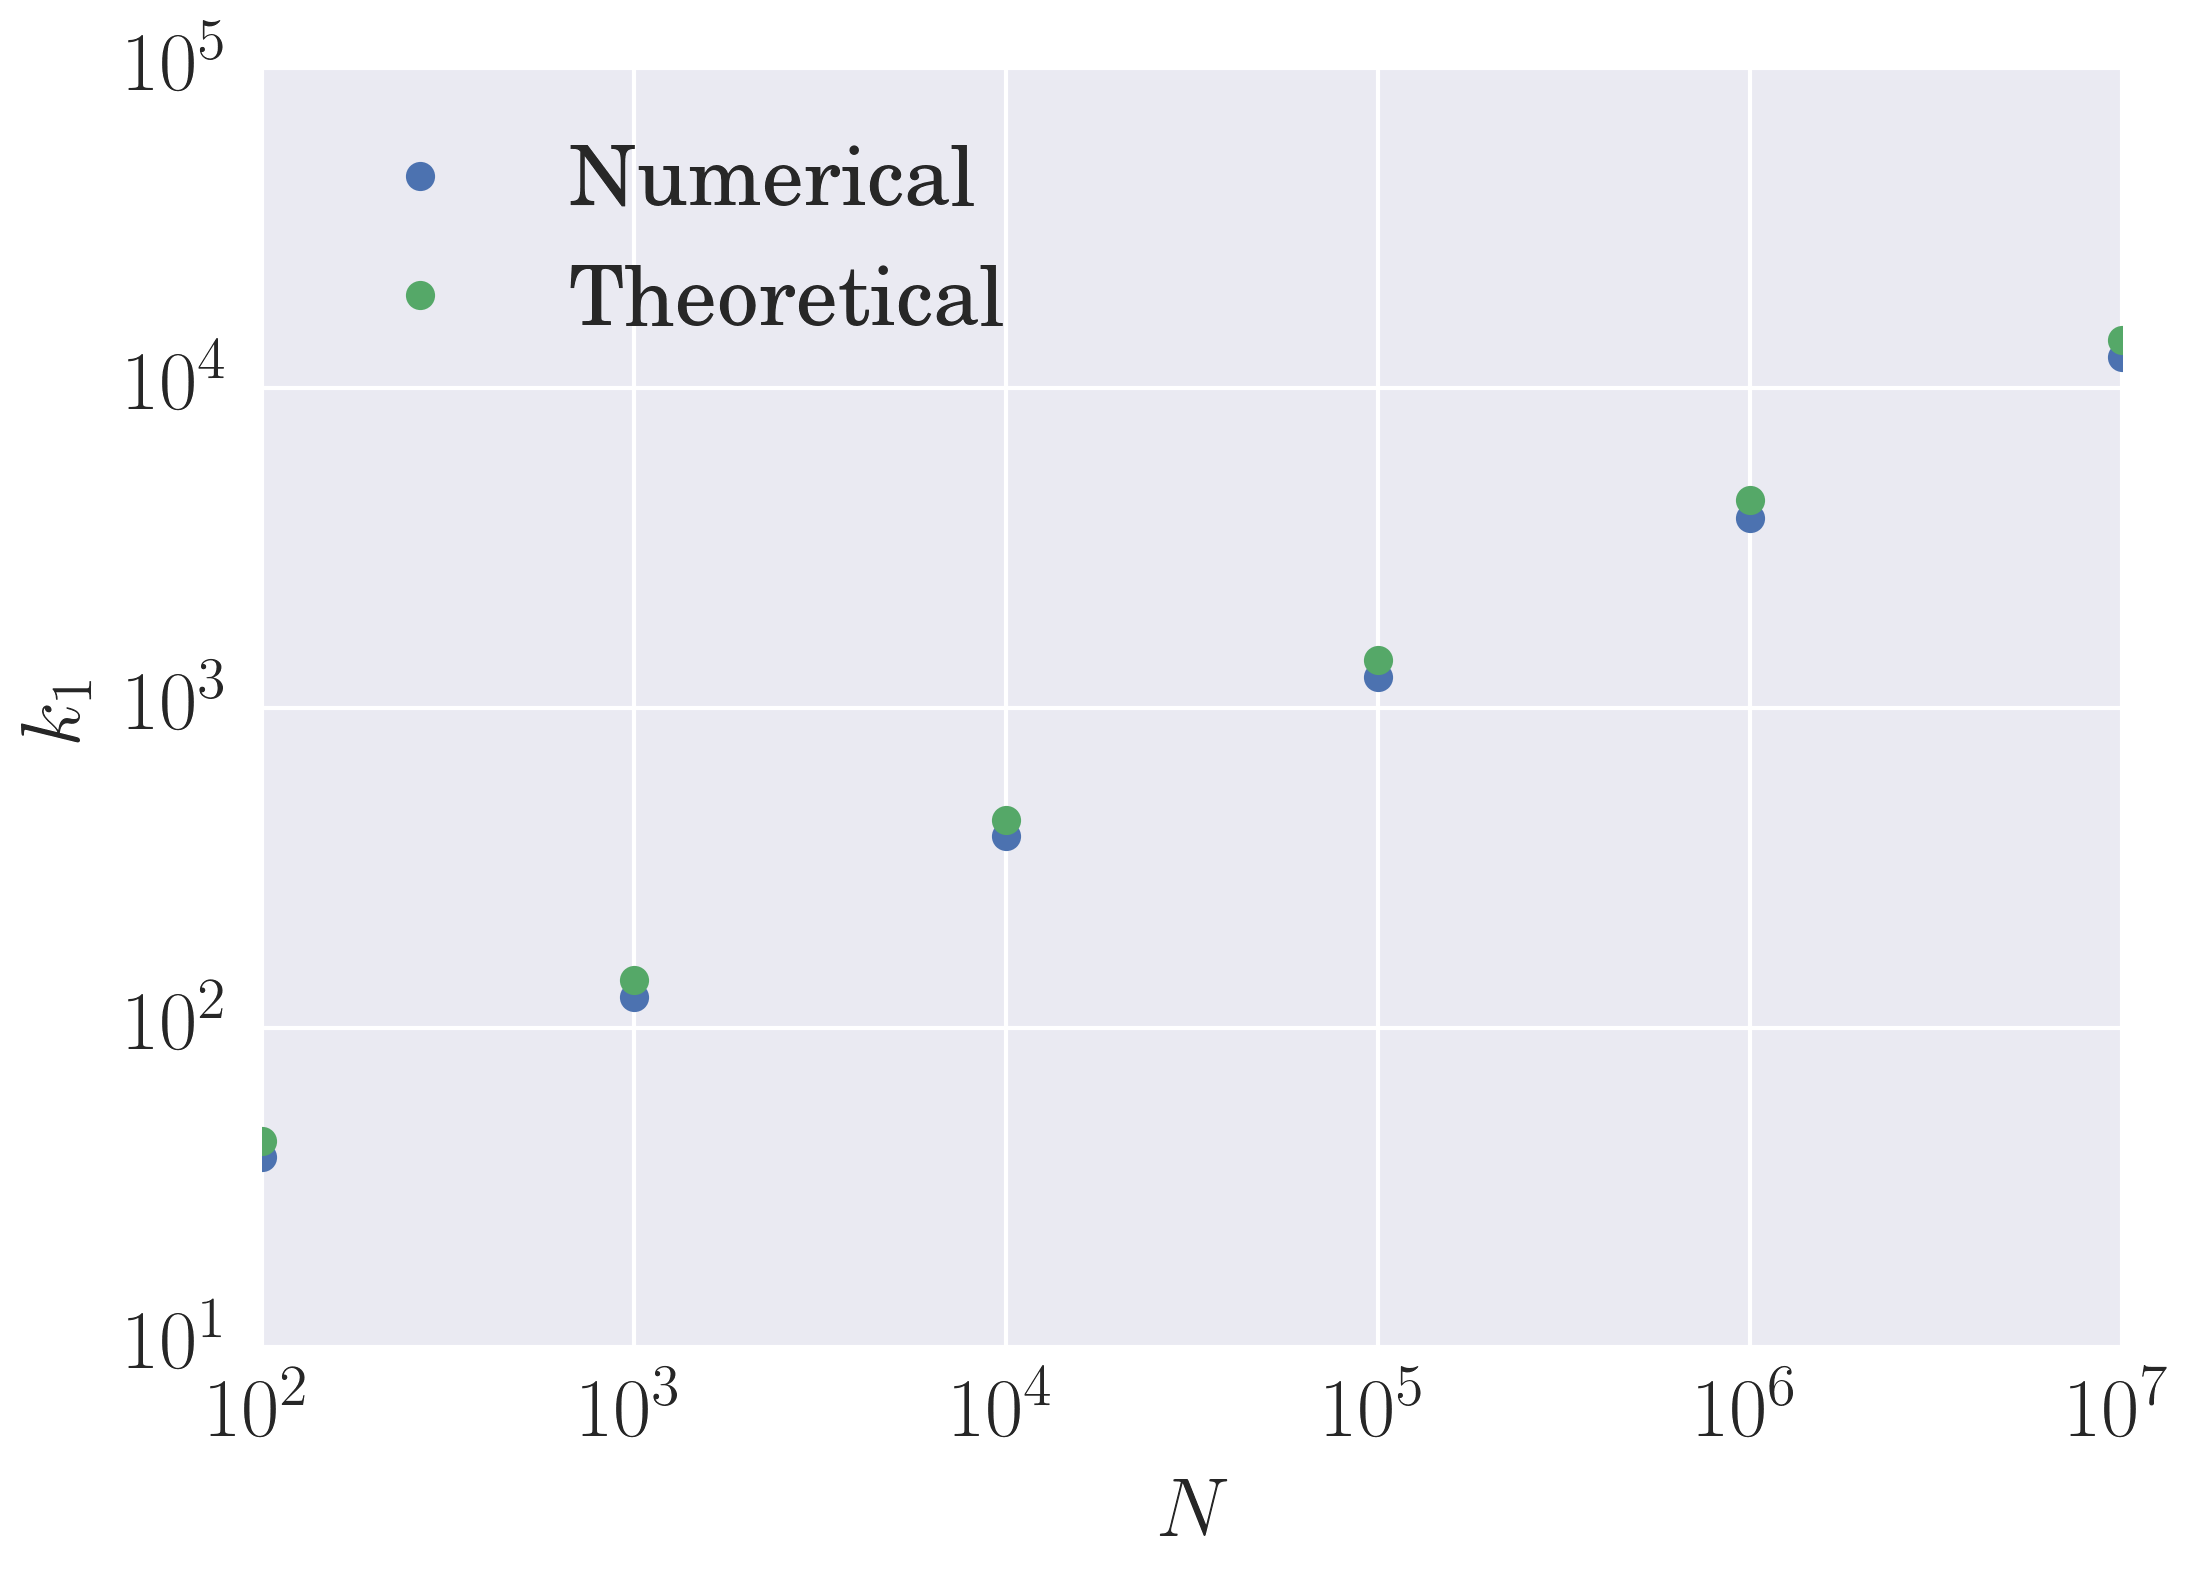
\includegraphics[height=0.5\linewidth]{img/pa-numerical-theoretical-k1}
    \caption{This shows the difference in $k_1$ for different values of $N$ ranging from $100$ to $10^7$ for preferential attachment. There is a constant offset of the numerical values from the theoretical, indicating a systematic bias instead of statistical fluctuations. }
    \label{fig:pa-numerical-theoretical-k1}
\end{figure}

\begin{center}
\begin{tabular}{ ||c | c | c | c ||}
\hline
N & $k_1^{\text{theory}}$ & $k_1^{\text{numerical}}$ & $k_1^{\text{numerical}} / k_1^{\text{theory}} $\\ 
\hline
$10^2$ & 45    & 39.3  $\pm$ 0.1 & 0.889 \\  
$10^3$ & 141   & 124.9 $\pm$ 0.3 & 0.886 \\
$10^4$ & 447   & 396   $\pm$  1  & 0.887 \\
$10^5$ & 1414  & 1248  $\pm$  3  & 0.883 \\
$10^6$ & 4472  & 3924  $\pm$  9  & 0.878 \\
$10^7$ & 14142 & 12558 $\pm$ 30  & 0.888 \\  
\hline
\end{tabular}
\label{table:pa-numerical-theoretical-ratio}
\captionof{table}{This table shows the theoretical and numerical values for the largest expected degree as defined in \autoref{eq:pa-k1-expression} for preferential attachment. The errors on $k_1$ are rounded off to 1 significant figure. }
\end{center}


To produce a data collapse, we need to find the function $f$ such that 

\begin{equation}
	p_N(k) = f(k) \mathcal{G}\left ( k / k_1 \right )
	\label{eq:data-collapse}
\end{equation}

To find $f(k)$, we know that in the limit of $N \rightarrow \infty$, $p$ must have no dependence on $L$, and in the large $N$ limit, $p_N(k) = f(k)$ which is just $p_{\infty}(k)$. This implies 
\begin{equation}
	\frac{p_N(k)}{p_{\infty}(k)} = G \left ( k / k_1 \right )
\end{equation}
which means that plotting $p_N(k) / p_{\infty}(k)$ against $k / k_1$ will produce a data collapse, as shown in \autoref{fig:pa-data-collapse}. 

\begin{figure}
    \centering
    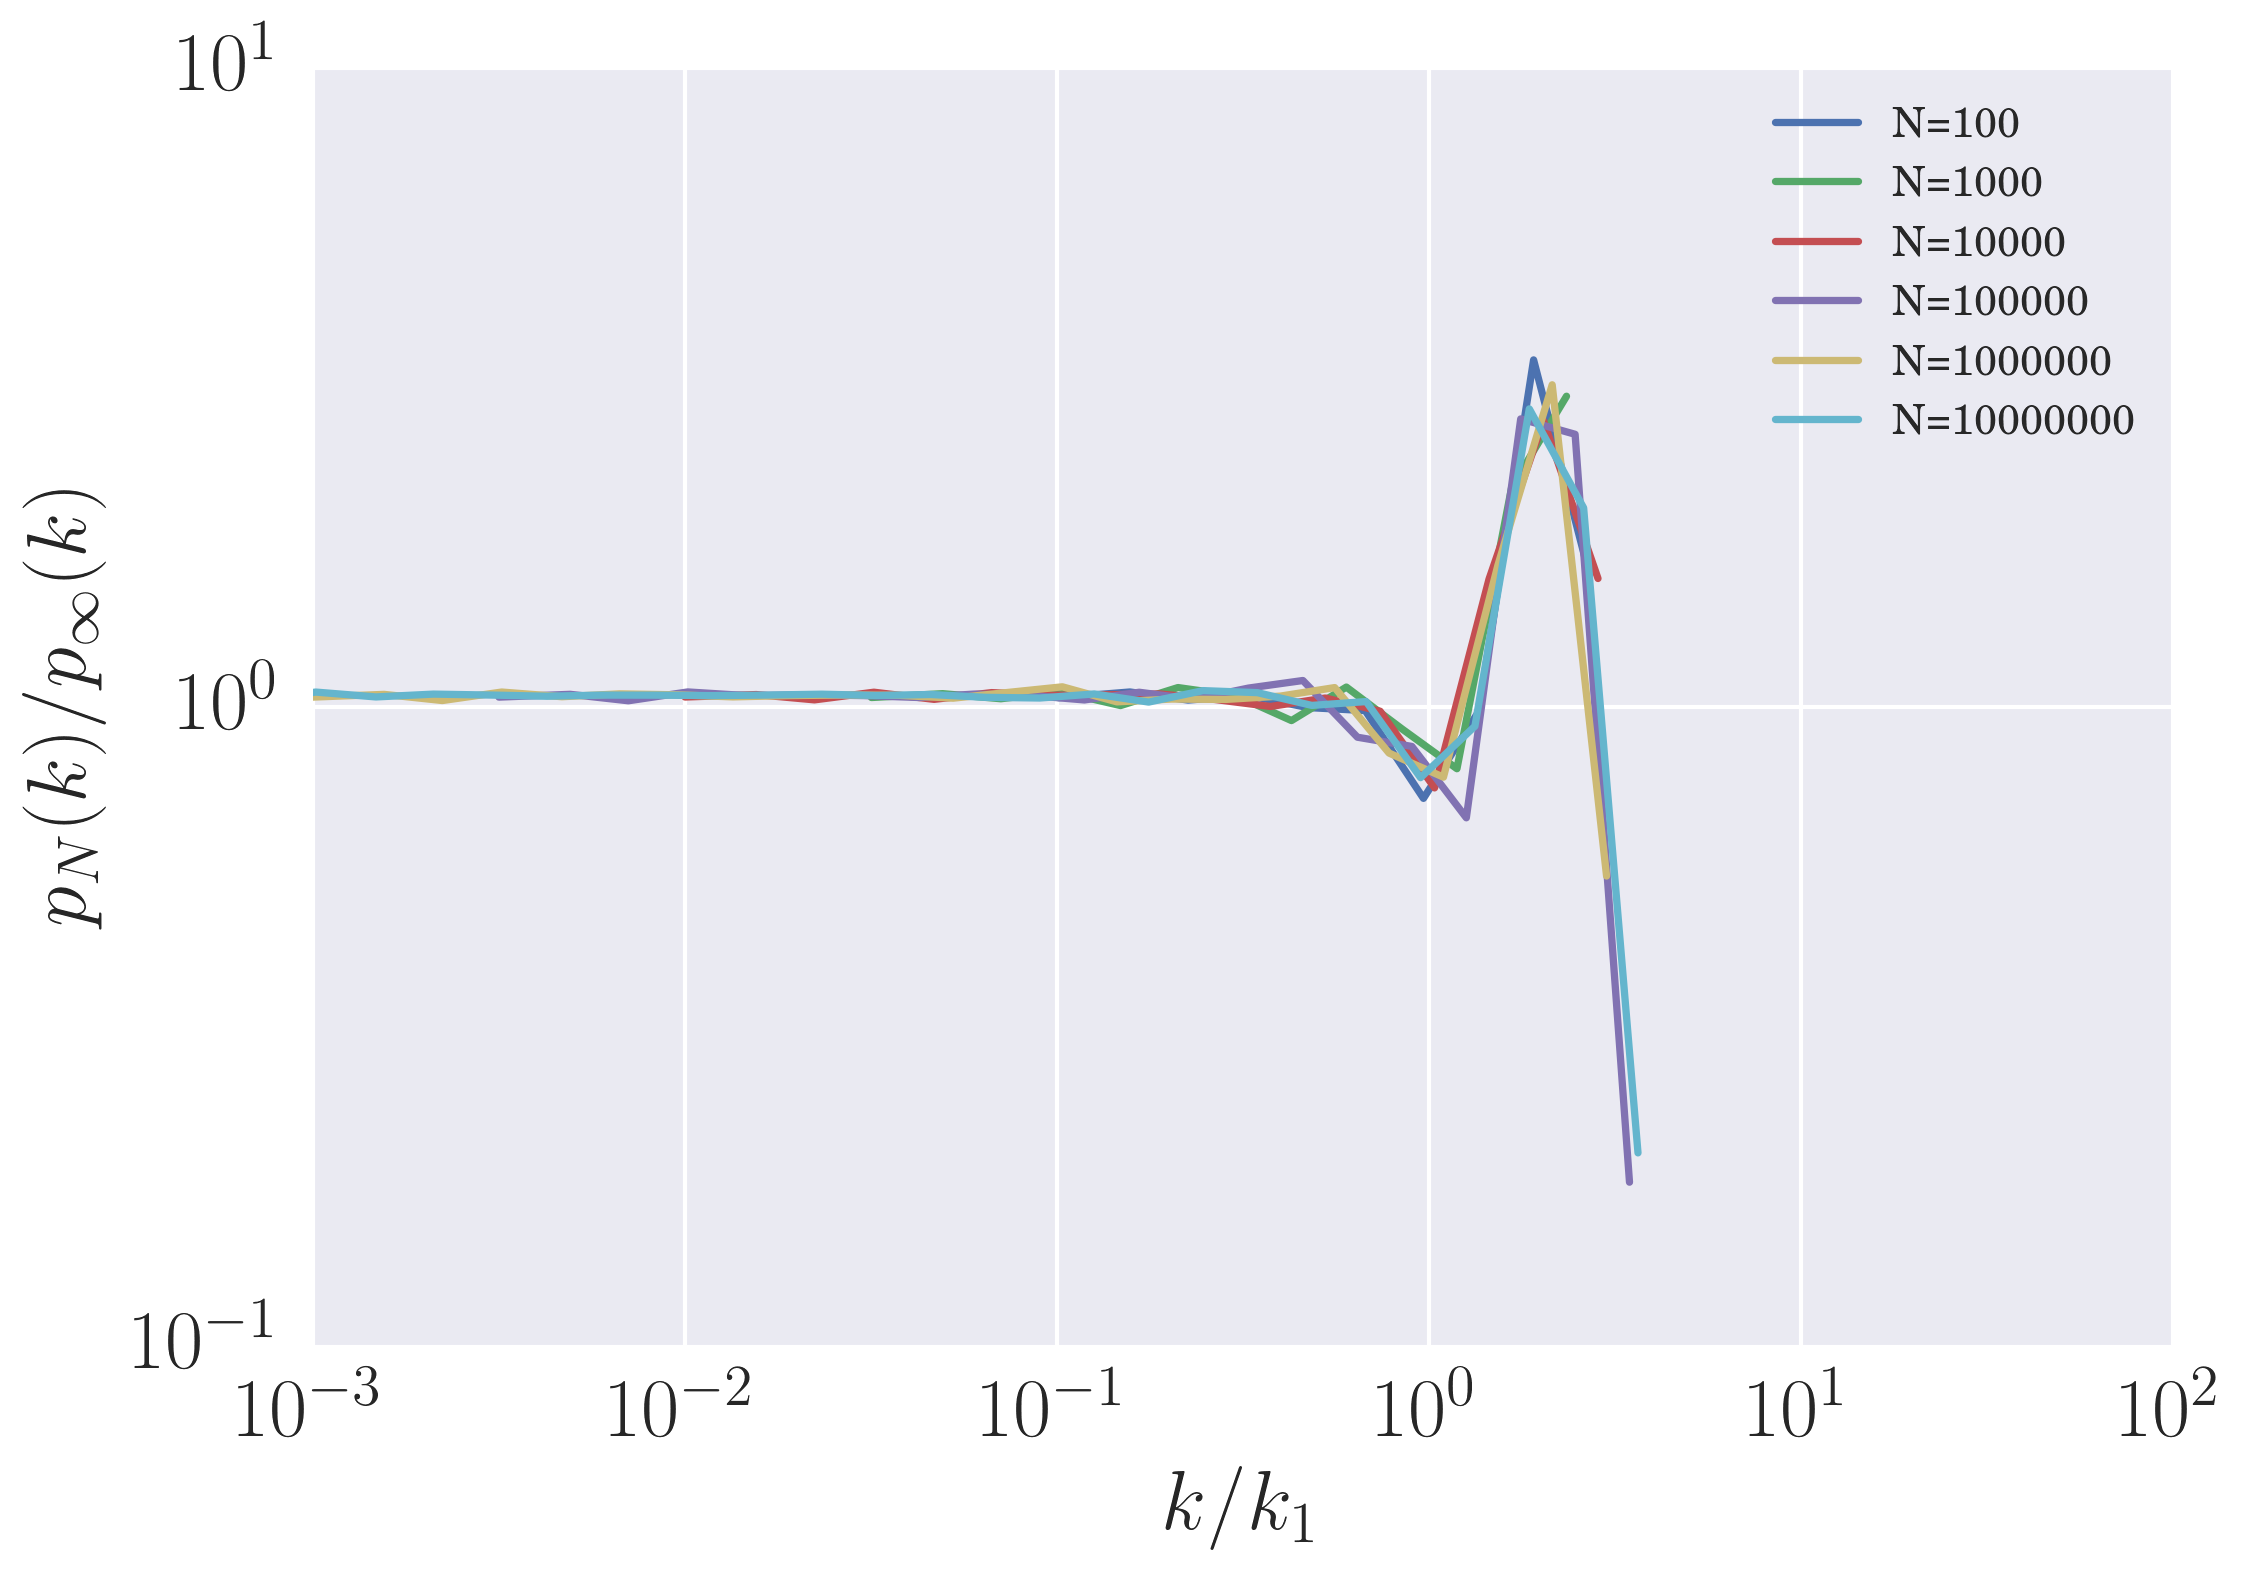
\includegraphics[height=0.5\linewidth]{img/pa-data-collapse}
    \caption{Data collapse of the degree distribution for networks of size $N=10^2, 10^3, 10^4, 10^5, 10^6, 10^7$}
    \label{fig:pa-data-collapse}
\end{figure}